% Created 2021-09-02 Thu 17:27
% Intended LaTeX compiler: pdflatex
\documentclass[presentation,aspectratio=169, usenames, dvipsnames]{beamer}
\usepackage[utf8]{inputenc}
\usepackage[T1]{fontenc}
\usepackage{graphicx}
\usepackage{grffile}
\usepackage{longtable}
\usepackage{wrapfig}
\usepackage{rotating}
\usepackage[normalem]{ulem}
\usepackage{amsmath}
\usepackage{textcomp}
\usepackage{amssymb}
\usepackage{capt-of}
\usepackage{hyperref}
\usepackage{khpreamble}
\usepackage{amssymb}
\usepgfplotslibrary{groupplots}
\newcommand*{\shift}{\operatorname{q}}
\definecolor{ppc}{rgb}{0.1,0.1,0.6}
\definecolor{iic}{rgb}{0.6,0.1,0.1}
\definecolor{ddc}{rgb}{0.1,0.6,0.1}
\usetheme{default}
\author{Kjartan Halvorsen}
\date{\today}
\title{Process Automation Laboratory - PID control}
\hypersetup{
 pdfauthor={Kjartan Halvorsen},
 pdftitle={Process Automation Laboratory - PID control},
 pdfkeywords={},
 pdfsubject={},
 pdfcreator={Emacs 26.3 (Org mode 9.4.6)}, 
 pdflang={English}}
\begin{document}

\maketitle

\section{Repetition - Second-order model critically damped}
\label{sec:orgd8c85bb}
\begin{frame}[label={sec:org8c495f4}]{Second-order models}
\end{frame}
\begin{frame}[label={sec:org4130cf8}]{Two first-order models in series}
\begin{center}
\begin{tikzpicture}
  \node {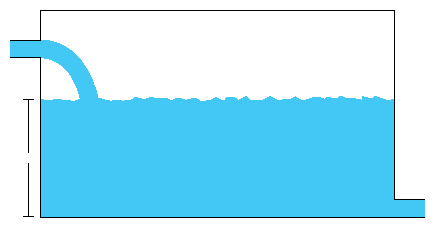
\includegraphics[width=0.4\linewidth]{../../figures/tank-with-hole-no-variables}};
  \node at (5.3,-2.05) {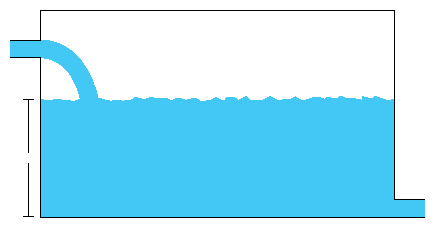
\includegraphics[width=0.4\linewidth]{../../figures/tank-with-hole-no-variables}};
\end{tikzpicture}
\end{center}

\begin{center}
  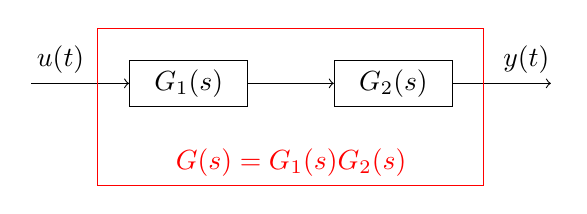
\begin{tikzpicture}[node distance=22mm, block/.style={rectangle, draw, minimum width=15mm}, sumnode/.style={circle, draw, inner sep=2pt}]

    \node[coordinate] (input) {};
    \node[block, right of=input, node distance=20mm] (plant1)  {$G_1(s)$};
    \node[block, right of=plant1, node distance=26mm] (plant2)  {$G_2(s)$};
    \node[coordinate, right of=plant2, node distance=20mm] (output) {};

    \draw[->] (input) -- node[above, pos=0.3] {$u(t)$} (plant1);
    \draw[->] (plant1) -- node[coordinate, ] (mp) { } (plant2);
    \draw[->] (plant2) -- node[above, near end] {$y(t)$} (output);
    \draw[red] (plant1.south west) ++(-4mm,-10mm) rectangle ++(49mm, 20mm);

    \node[red,below of=mp, node distance=10mm] {$G(s) = G_1(s)G_2(s)$};
  \end{tikzpicture}
\end{center}
\end{frame}


\begin{frame}[label={sec:org51bc4e6}]{Fitting second-order critically-damped model}
\alert{Model with two identical time-constants.}
Assuming model 
\[ \textcolor{green!50!black}{Y(s)} = \frac{K}{(s\tau + 1)^2}\textcolor{blue!80!black}{U(s)} \quad \overset{U(s) = \frac{u_f}{s}}{\Longrightarrow} \quad \textcolor{green!50!black}{y(t)} = u_f K\Big( 1 - (1+\frac{t}{\tau}\big)\mathrm{e}^{-\frac{t}{\tau}}\Big)u_H(t)\]
\def\Tcnst{2}
\def\tdelay{0.0}
\def\ggain{2}
\def\uampl{0.8}
\pgfmathsetmacro{\yfinal}{\uampl*\ggain}
\pgfmathsetmacro{\ytwo}{\yfinal*(1-2*exp(-1))}
\pgfmathsetmacro{\ytwofactor}{(1-2*exp(-1))}
\pgfmathsetmacro{\two}{\tdelay + \Tcnst}

\begin{center}
  \begin{tikzpicture}
    \begin{axis}[
    width=14cm,
    height=4.5cm,
    grid = both,
    xtick = {0, \two},
    xticklabels = {0,  $\tau$},
    ytick = {0, \ytwo, \uampl, \yfinal},
    yticklabels = {0, $\ytwofactor y_f$, $u_f$, $y_f$},
    xmin = -0.2,
    clip = false,
    %minor y tick num=9,
    %minor x tick num=9,
    %every major grid/.style={red, opacity=0.5},
    ]
      \addplot [thick, green!50!black, no marks, domain=0:11, samples=100] {\uampl*\ggain*(x>\tdelay)*(1 - (1+x/\Tcnst)*exp(-(x-\tdelay)/\Tcnst)} node [coordinate, pos=0.9, pin=-90:{$y(t)$}] {};
      \addplot [const plot, thick, blue!80!black, no marks, domain=-1:11, samples=100] coordinates {(-1,0) (0,0) (0,\uampl) (11,\uampl)} node [coordinate, pos=0.9, pin=-90:{$u(t)$}] {};
      \node at (axis cs: 11, -0.3) {$t$};
    \end{axis}
  \end{tikzpicture}
\end{center}

\[ y_f = \lim_{t\to\infty} y(t) = u_f K \quad \Rightarrow \quad K = \frac{y_f}{u_f}. \]
\end{frame}


\section{PID parameter intuition}
\label{sec:org9124c70}
\begin{frame}[label={sec:org21ee677}]{Feedback control}
   \begin{center}
   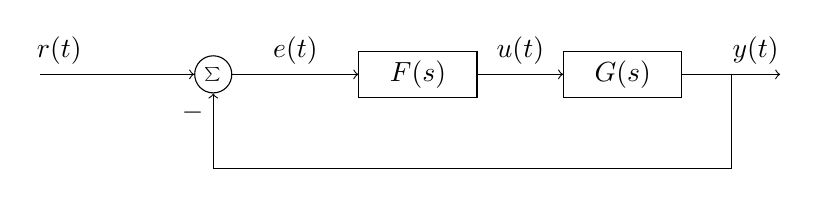
\begin{tikzpicture}[node distance=22mm, block/.style={rectangle, draw, minimum width=15mm}, sumnode/.style={circle, draw, inner sep=2pt}]
  { 
  \node[coordinate] (input) {};
  \node[sumnode, right of=input] (sum) {\tiny $\sum$};
  \node[block, right of=sum, node distance=2.6cm] (reg) {$F(s)$};
  \node[block, right of=reg, node distance=2.6cm] (plant) {$G(s)$};
  \node[coordinate, right of=plant, node distance=2cm] (output) {};
  \node[coordinate, below of=plant, node distance=12mm] (feedback) {};
 
  \draw[->] (plant) -- node[coordinate, inner sep=0pt] (meas) {} node[near end, above] {$y(t)$} (output);
  \draw[->] (meas) |- (feedback) -| node[very near end, left] {$-$} (sum);
  \draw[->] (input) -- node[very near start, above] {$r(t)$} (sum);
  \draw[->] (sum) -- node[above] {$e(t)$} (reg);
  \draw[->] (reg) -- node[above] {$u(t)$}(plant);
}
\end{tikzpicture}
\end{center}
\end{frame}



\begin{frame}[label={sec:org2fb2529}]{The PID controller}
\begin{center}
  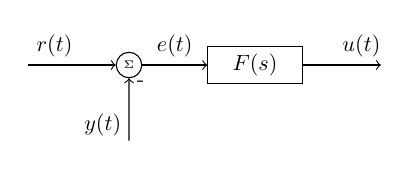
\begin{tikzpicture}[node distance=22mm, block/.style={rectangle, draw, minimum width=15mm}, sumnode/.style={circle, draw, inner sep=2pt},scale=0.8, every node/.style={scale=0.8}]

    \node[coordinate] (input) {};
    \node[sumnode, right of=input, node distance=16mm] (sum) {\tiny $\Sigma$};
    \node[block, right of=sum, node distance=20mm] (pid)  {$F(s)$};
    \node[coordinate, below of=sum, node distance=12mm] (feedback) {};
    \node[coordinate, right of=pid, node distance=20mm] (output) {};

    \draw[->] (input) -- node[above, pos=0.3] {$r(t)$} (sum);
    \draw[->] (sum) -- node[above] {$e(t)$} (pid);
    \draw[->] (pid) -- node[above, near end] {$u(t)$} (output);
    \draw[->] (feedback) -- node[left, near start] {$y(t)$} node[right, pos=0.95] {-} (sum);
  \end{tikzpicture}
\end{center}

\alert{Parallel form (ISA)}
\[   F(s) &= k_c\left( 1 + \frac{1}{\tau_i s} + \tau_d s\right) \]

\alert{Series form}
\[F(s) = K_c \left( \frac{ \tau_I s + 1}{\tau_I s} \right) (\tau_D s + 1) 
= \underbrace{\frac{K_c(\tau_I + \tau_D)}{\tau_I}}_{k_c} \left(1 + \frac{1}{\underbrace{(\tau_I + \tau_D)}_{\tau_i} s} + \underbrace{\frac{\tau_I\tau_D}{\tau_I + \tau_D}}_{\tau_d}s \right) \]
\end{frame}


\begin{frame}[label={sec:orgae39394}]{The PID - Parallel form}
\definecolor{ppc}{rgb}{0.1,0.1,0.6}
\definecolor{iic}{rgb}{0.6,0.1,0.1}
\definecolor{ddc}{rgb}{0.1,0.6,0.1}

\begin{center}
  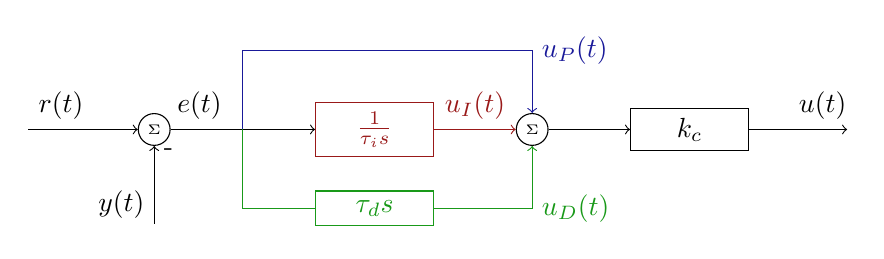
\begin{tikzpicture}[node distance=22mm, block/.style={rectangle, draw, minimum width=15mm}, sumnode/.style={circle, draw, inner sep=2pt}]

    \node[coordinate] (input) {};
    \node[sumnode, right of=input, node distance=16mm] (sum) {\tiny $\Sigma$};
    \node[color=iic,block, right of=sum, node distance=28mm] (ii)  {$\frac{1}{\tau_is}$};
    \node[color=ppc, coordinate, above of=ii, node distance=10mm] (pp)  {};
    \node[color=ddc,block, below of=ii, node distance=10mm] (dd)  {$\tau_ds$};
    \node[sumnode, right of=ii, node distance=20mm] (sum2) {\tiny $\Sigma$};
    \node[block, right of=sum2, node distance=20mm] (gain)  {$k_c$};
    \node[coordinate, below of=sum, node distance=12mm] (feedback) {};
    \node[coordinate, right of=gain, node distance=20mm] (output) {};

    \draw[->] (input) -- node[above, pos=0.3] {$r(t)$} (sum);
    \draw[->] (sum) -- node[above, pos=0.2] {$e(t)$} node[coordinate] (mm) {}  (ii);
    \draw[->] (gain) -- node[above, near end] {$u(t)$} (output);
    \draw[->] (feedback) -- node[left, near start] {$y(t)$} node[right, pos=0.95] {-} (sum);
    \draw[->, color=ppc] (mm) |- (pp) -| node[right,] {$u_P(t)$} (sum2);
    \draw[->, color=ddc] (mm) |- (dd) -| node[right,] {$u_D(t)$} (sum2);
    \draw[->, color=iic] (ii)  -- node[above,] {$u_I(t)$} (sum2);
    \draw[->] (sum2) -- node[above, near end] {} (gain);

  \end{tikzpicture}
\end{center}

\begin{align*}
u(t) &= k_c\Big( \textcolor{ppc}{e(t)} + \textcolor{iic}{\frac{1}{\tau_i} \int_0^{t} e(\xi) d\xi} + \textcolor{ddc}{\tau_d \frac{d}{dt} e(t)} \Big)
\end{align*}
\end{frame}

\begin{frame}[label={sec:orga5afc99}]{The PID - Parallel form, modified D-part}
\definecolor{ppc}{rgb}{0.1,0.1,0.6}
\definecolor{iic}{rgb}{0.6,0.1,0.1}
\definecolor{ddc}{rgb}{0.1,0.6,0.1}

\begin{center}
  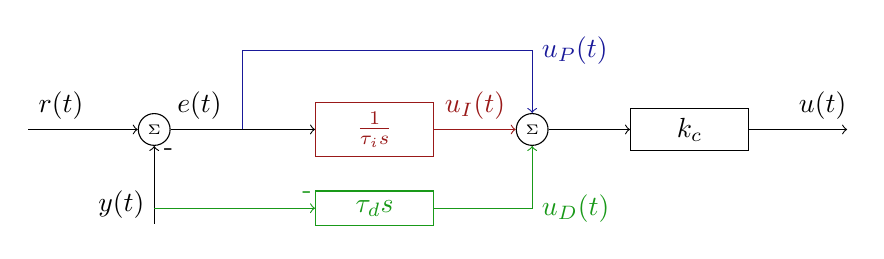
\begin{tikzpicture}[node distance=22mm, block/.style={rectangle, draw, minimum width=15mm}, sumnode/.style={circle, draw, inner sep=2pt}]

    \node[coordinate] (input) {};
    \node[sumnode, right of=input, node distance=16mm] (sum) {\tiny $\Sigma$};
    \node[color=iic,block, right of=sum, node distance=28mm] (ii)  {$\frac{1}{\tau_is}$};
    \node[color=ppc, coordinate, above of=ii, node distance=10mm] (pp)  {};
    \node[color=ddc,block, below of=ii, node distance=10mm] (dd)  {$\tau_ds$};
    \node[sumnode, right of=ii, node distance=20mm] (sum2) {\tiny $\Sigma$};
    \node[block, right of=sum2, node distance=20mm] (gain)  {$k_c$};
    \node[coordinate, below of=sum, node distance=12mm] (feedback) {};
    \node[coordinate, right of=gain, node distance=20mm] (output) {};

    \draw[->] (input) -- node[above, pos=0.3] {$r(t)$} (sum);
    \draw[->] (sum) -- node[above, pos=0.2] {$e(t)$} node[coordinate] (mm) {}  (ii);
    \draw[->] (gain) -- node[above, near end] {$u(t)$} (output);
    \draw[->] (feedback) -- node[left, near start] {$y(t)$} node[right, pos=0.95] {-} (sum);
    \draw[->, color=ppc] (mm) |- (pp) -| node[right,] {$u_P(t)$} (sum2);
    \draw[->, color=ddc] (feedback |- dd) -- node[above, pos=0.95] {-} (dd);
    \draw[->, color=ddc] (dd) -| node[right,] {$u_D(t)$} (sum2)  ;
    \draw[->, color=iic] (ii)  -- node[above,] {$u_I(t)$} (sum2);
    \draw[->] (sum2) -- node[above, near end] {} (gain);

  \end{tikzpicture}
\end{center}

\[    u(t) = k_c\Big( \textcolor{ppc}{e(t)} + \textcolor{iic}{\overbrace{\frac{1}{\tau_i} \int_0^{t} e(\xi) d\xi}^{u_I(t)}} + \textcolor{ddc}{ \underbrace{\tau_d \frac{d}{dt} \big(-y(t)\big)}_{u_D(t)}} \Big) \]
\end{frame}

\begin{frame}[label={sec:org320807c}]{The PID - Parallel form}
\begin{center}
  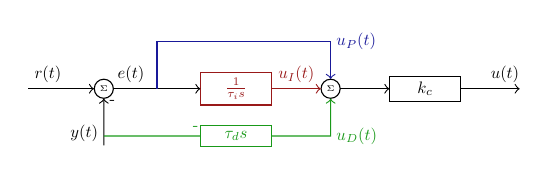
\begin{tikzpicture}[node distance=22mm, block/.style={rectangle, draw, minimum width=15mm}, sumnode/.style={circle, draw, inner sep=2pt}, scale=0.6, every node/.style={scale=0.6}]

    \node[coordinate] (input) {};
    \node[sumnode, right of=input, node distance=16mm] (sum) {\tiny $\Sigma$};
    \node[color=iic,block, right of=sum, node distance=28mm] (ii)  {$\frac{1}{\tau_is}$};
    \node[color=ppc, coordinate, above of=ii, node distance=10mm] (pp)  {};
    \node[color=ddc,block, below of=ii, node distance=10mm] (dd)  {$\tau_ds$};
    \node[sumnode, right of=ii, node distance=20mm] (sum2) {\tiny $\Sigma$};
    \node[block, right of=sum2, node distance=20mm] (gain)  {$k_c$};
    \node[coordinate, below of=sum, node distance=12mm] (feedback) {};
    \node[coordinate, right of=gain, node distance=20mm] (output) {};

    \draw[->] (input) -- node[above, pos=0.3] {$r(t)$} (sum);
    \draw[->] (sum) -- node[above, pos=0.2] {$e(t)$} node[coordinate] (mm) {}  (ii);
    \draw[->] (gain) -- node[above, near end] {$u(t)$} (output);
    \draw[->] (feedback) -- node[left, near start] {$y(t)$} node[right, pos=0.95] {-} (sum);
    \draw[->, color=ppc] (mm) |- (pp) -| node[right,] {$u_P(t)$} (sum2);
    \draw[->, color=ddc] (feedback |- dd) -- node[above, pos=0.95] {-} (dd) -| node[right,] {$u_D(t)$}   (sum2);
    \draw[->, color=iic] (ii)  -- node[above,] {$u_I(t)$} (sum2);
    \draw[->] (sum2) -- node[above, near end] {} (gain);

  \end{tikzpicture}
  \small
  \(  u(t) = k_c\Big( \textcolor{ppc}{e(t)} + \textcolor{iic}{\overbrace{\frac{1}{\tau_i} \int_0^{t} e(\xi) d\xi}^{u_I(t)}} + \textcolor{ddc}{ \underbrace{\tau_d \frac{d}{dt} \big(-y(t)\big)}_{u_D(t)}} \Big)\)
\end{center}

   \begin{center}
   \def\TT{1}
   \begin{tikzpicture}
   \begin{axis}[
    clip=false,
    width=14cm,
    height=4.5cm,
    ylabel={},
    xlabel={$t$},
    ymax = 2,
    ymin = -0.5,
    ]
      \addplot[black, no marks, domain=-0.1:8, samples=200] {(x>0)*(1 - (1+x/\TT)*exp(-x/\TT)} node[coordinate, pin=-20:{$y(t)$}, pos=0.4] {};
      \addplot[magenta!70!black, no marks, domain=-0.1:8, samples=200] coordinates {(-0.1, 0) (0,0) (0,1) (8,1)} node[coordinate, pin=90:{$r(t)$}, pos=0.4] {};
    \end{axis}

 \end{tikzpicture}
\end{center}
\alert{Activity} Sketch the error signal \(e(t)\), the derivative signal \(u_D(t)\) and the integral signal \(u_I(t)\) (use \(\tau_i=\tau_d=1\))
\end{frame}

\begin{frame}[label={sec:org0429488}]{The PID - Parallel form, solution}
\end{frame}
\begin{frame}[label={sec:orgb2e7e1a}]{The PID - Parallel form, solution}
\(u(t) = k_c\Big( \textcolor{ppc}{e(t)} + \textcolor{iic}{\overbrace{\frac{1}{\tau_i} \int_0^{t} e(\xi) d\xi}^{u_I(t)}} + \textcolor{ddc}{ \underbrace{\tau_d \frac{d}{dt} \big(-y(t)\big)}_{u_D(t)}} \Big)\)
   \begin{center}
   \def\TT{1}
   \begin{tikzpicture}
   \begin{axis}[
    clip=false,
    width=14cm,
    height=5cm,
    ylabel={},
    xlabel={$t$},
    ymax = 2,
    ]
      \addplot[black, no marks, domain=-0.1:8, samples=200] {(x>0)*(1 - (1+x/\TT)*exp(-x/\TT)} node[coordinate, pin=-20:{$y(t)$}, pos=0.4] {};
      \addplot[magenta!70!black, no marks, domain=-0.1:8, samples=200] coordinates {(-0.1, 0) (0,0) (0,1) (8,1)} node[coordinate, pin=90:{$r(t)$}, pos=0.21] {};
      \addplot[color=ppc, no marks, domain=0:8, samples=200] {(x>=0)*( (1+x/\TT)*exp(-x/\TT)} node[coordinate, pin=20:{$e(t)$}, pos=0.7] {};
      \addplot[color=iic, no marks, domain=-0.1:8, samples=200] {(x>0)*(2*(1-exp(-x/\TT)) - \x/\TT*exp(-x/\TT))} node[coordinate, pin=-20:{$u_I(t)$}, pos=0.6] {};
      \addplot[color=ddc, no marks, domain=-0.1:8, samples=200] {(x>0)*(-\x/\TT*exp(-x/\TT))} node[coordinate, pin=-20:{$u_D(t)$}, pos=0.4] {};
    \end{axis}

 \end{tikzpicture}
\end{center}
\end{frame}

\begin{frame}[label={sec:org586fa5e}]{The PID - practical form}
\definecolor{ppc}{rgb}{0.1,0.1,0.6}
\definecolor{iic}{rgb}{0.6,0.1,0.1}
\definecolor{ddc}{rgb}{0.1,0.5,0.1}

\begin{center}
  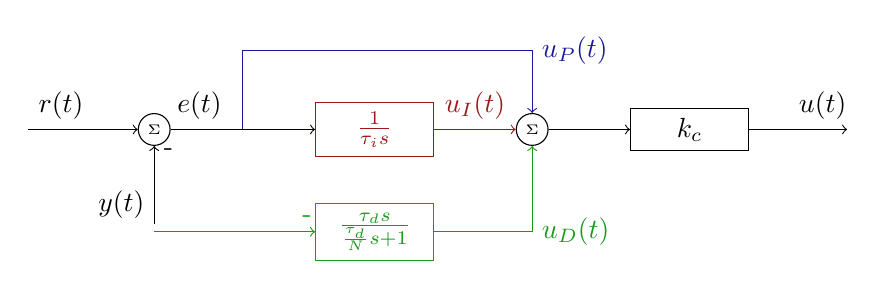
\begin{tikzpicture}[node distance=22mm, block/.style={rectangle, draw, minimum width=15mm}, sumnode/.style={circle, draw, inner sep=2pt}]

    \node[coordinate] (input) {};
    \node[sumnode, right of=input, node distance=16mm] (sum) {\tiny $\Sigma$};
    \node[color=iic,block, right of=sum, node distance=28mm] (ii)  {$\frac{1}{\tau_is}$};
    \node[color=ppc, coordinate, above of=ii, node distance=10mm] (pp)  {};
    \node[color=ddc,block, below of=ii, node distance=13mm] (dd)  {$\frac{\tau_ds}{\frac{\tau_d}{N}s + 1}$};
    \node[sumnode, right of=ii, node distance=20mm] (sum2) {\tiny $\Sigma$};
    \node[block, right of=sum2, node distance=20mm] (gain)  {$k_c$};
    \node[coordinate, below of=sum, node distance=12mm] (feedback) {};
    \node[coordinate, right of=gain, node distance=20mm] (output) {};

    \draw[->] (input) -- node[above, pos=0.3] {$r(t)$} (sum);
    \draw[->] (sum) -- node[above, pos=0.2] {$e(t)$} node[coordinate] (mm) {}  (ii);
    \draw[->] (gain) -- node[above, near end] {$u(t)$} (output);
    \draw[->] (feedback) -- node[left, near start] {$y(t)$} node[right, pos=0.95] {-} (sum);
    \draw[->, color=ppc] (mm) |- (pp) -| node[right,] {$u_P(t)$} (sum2);
    \draw[->, color=ddc] (feedback |- dd) -- node[above, pos=0.95] {-} (dd);
    \draw[->, color=ddc] (dd) -| node[right,] {$u_D(t)$} (sum2)  ;
    \draw[->, color=iic] (ii)  -- node[above,] {$u_I(t)$} (sum2);
    \draw[->] (sum2) -- node[above, near end] {} (gain);

  \end{tikzpicture}
\end{center}

The parameter \(N\) is chosen to limit the influence of noisy measurements. Typically,
\[  3 < N < 10 \]
\end{frame}

\section{PID tuning - (Smith and Corripio) Ziegler Nichols}
\label{sec:orga158d8d}
\begin{frame}[label={sec:orgd1f6a5d}]{PID tuning}
\end{frame}
\begin{frame}[label={sec:org71a4d7d}]{Method by Smith \& Corripio using table by Ziegler-Nichols}
\small

Given process model (fitted to response of the system) \[ G(s) = K \frac{\mathrm{e}^{-s\theta}}{\tau s + 1} \] and PID controller
   \[ F(s) = k_c\left( 1 + \frac{1}{\tau_i s} + \tau_d s\right) \]
   Choose the PID parameters according to the following table (Ziegler-Nichols, 1943)
   \begin{center}
   \setlength{\tabcolsep}{20pt}
   \renewcommand{\arraystretch}{1.5}
   \begin{tabular}{llll}
   Controller & \(k_c\) & \(\tau_i\) & \(\tau_d\)\\
  \hline\hline
  P & \(\frac{\tau}{\theta K}\) &  & \\
  PI & \(\frac{0.9\tau}{\theta K}\) & \(\frac{\theta}{0.3}\) & \\
  PID & \(\frac{1.2\tau}{\theta K}\) & \(2\theta\) & \(\frac{\theta}{2}\)\\
  \hline
\end{tabular}
\end{center}

Gives good control for \[0.1 < \frac{\theta}{\tau} < 0.6.\]
\end{frame}



\section{SIMC}
\label{sec:org627d95f}

\begin{frame}[label={sec:org62fb5a1}]{SIMC-PID tuning rule}
[ SIMC stands for \emph{SIMple Control} or \emph{Skogestad Internal Model Control} ]
   \begin{center}
   \begin{tikzpicture}[node distance=22mm, block/.style={rectangle, draw, minimum width=15mm}, sumnode/.style={circle, draw, inner sep=2pt}scale=0.5, every node/.style={scale=0.5}]
  { 
  \node[coordinate] (input) {};
  \node[sumnode, right of=input] (sum) {\tiny $\sum$};
  \node[block, right of=sum, node distance=2.6cm] (reg) {$F(s)$};
  \node[block, right of=reg, node distance=2.6cm] (plant) {$G(s)$};
  \node[coordinate, right of=plant, node distance=2cm] (output) {};
  \node[coordinate, below of=plant, node distance=12mm] (feedback) {};
 
  \draw[->] (plant) -- node[coordinate, inner sep=0pt] (meas) {} node[near end, above] {$y(t)$} (output);
  \draw[->] (meas) |- (feedback) -| node[very near end, left] {$-$} (sum);
  \draw[->] (input) -- node[very near start, above] {$r(t)$} (sum);
  \draw[->] (sum) -- node[above] {$e(t)$} (reg);
  \draw[->] (reg) -- node[above] {$u(t)$}(plant);
}
\end{tikzpicture}
\end{center}

Given model of the process and desired closed-loop system \[G(s) = K \frac{\mathrm{e}^{-s\theta}}{(\tau_1 s + 1)(\tau_2 s + 1)}, \quad \tau_1 \ge \tau_2; \qquad G_c(s) = \frac{\mathrm{e}^{-s\theta}}{\tau_c s + 1} \] Good robustness is obtained with PID controller

\[F(s) = K_c \left( \frac{ \tau_I s + 1}{\tau_I s} \right) (\tau_d s + 1) 
= \frac{K_c(\tau_I + \tau_d)}{\tau_I} \left(1 + \frac{1}{(\tau_I + \tau_D) s} + \frac{\tau_I\tau_D}{\tau_I + \tau_D}s \right) \]
with 
\[ K_c = \frac{\tau_1}{K(\tau_c + \theta)}, \qquad \tau_I = \min\{\tau_1, 4(\tau_c + \theta)\}, \qquad \tau_d = \tau_2 \]
\end{frame}
\end{document}